\section{Loading a Kernel}
Host programs can upload kernels to the GPU, and should preferably do so at the beginning of the program, to avoid delays during execution.
The CPU has a built-in function for this called \verb/load_kernel/\ref{lst:load-kernel}.
It takes an array of assembled instructions as parameter and returns a reference to GPU memory.
This reference can be used when setting kernel parameters and starting kernels.

\begin{c-code}[caption=A load\_kernel function call with the fillscreen kernel, label=lst:load-kernel]
kernel_t fill_screen = load_kernel(fill_screen_kernel);
\end{c-code}

The \verb/load_kernel/ function is implemented by maintaining an internal counter of used instruction memory on the GPU.
All kernels must end with the \verb/thread_finished/ instruction,
and the load function will keep loading until this instruction is reached.
The function returns the address of the first instruction, and increments the counter to reflect the next starting point.

\begin{figure}[H]
    \centering
    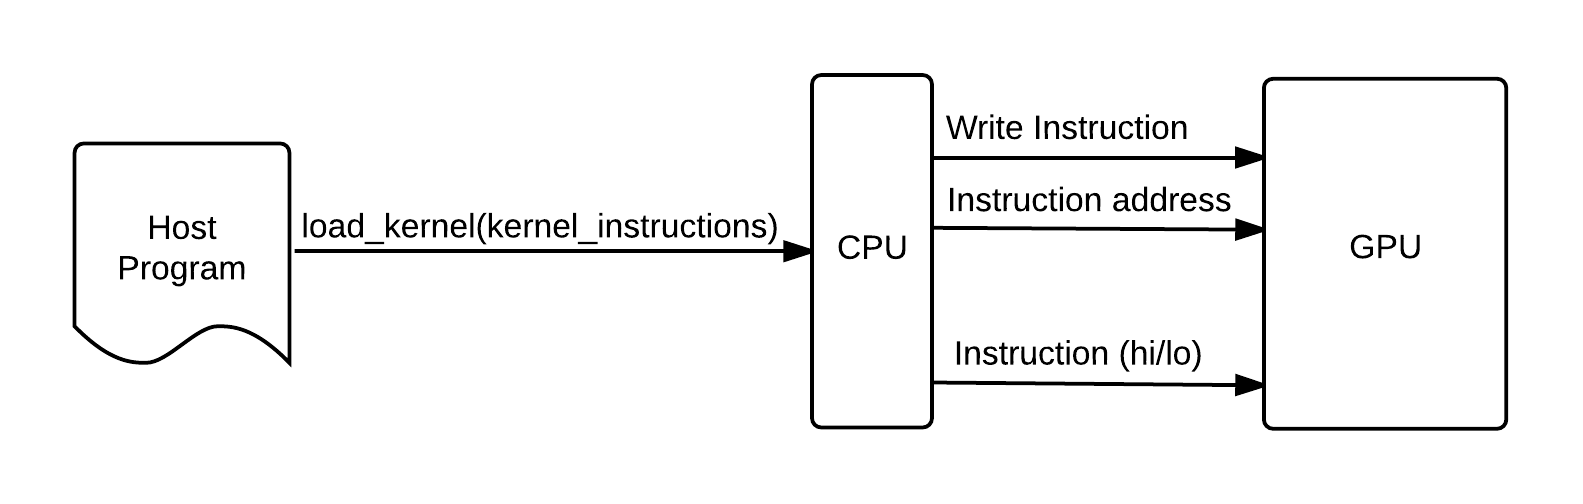
\includegraphics[width=\textwidth]{../cpu/diagrams/loading_a_kernel.png}
    \caption{}
    \label{fig:loading_a_kernel}
\end{figure}

Seeing as instructions are 32-bit large, and the data bus is only 16 bits,
every instruction load must be divided in two writes.
This is indicated by the hi\_select bit in the address format, as seen in figure \ref{fig:load_instruction_format}

\begin{figure}[H]
    \centering
    \begin{tabular}{|c|c|c|c|c|}
    \multicolumn{1}{c}{1} & \multicolumn{1}{c}{1} & \multicolumn{1}{c}{1} & \multicolumn{1}{c}{16}  & \multicolumn{1}{c}{1} \\ \hline
    X & 0 & 1 & address & hi\_select \\ \hline
    \end{tabular}
    \caption{Address format for loading an instruction.}
    \label{fig:load_instruction_format}
\end{figure}
